\documentclass{article}

% import packages
\usepackage{amsmath,amsfonts,amsthm,amssymb,amsopn,bm}
\usepackage{mathtools}
\usepackage[margin=.9in]{geometry}
\usepackage{graphicx}
\usepackage[dvipsnames]{xcolor}
\usepackage{minted}
\usepackage{subcaption}
\usepackage{float}

% note command
\newcommand{\note}[1]{\textsf{\textcolor{Red}{#1}}}

% some math commands
\newcommand{\norm}[1]{\left\|#1\right\|}
\newcommand{\twonorm}[1]{\|#1\|_2^2}
\newcommand{\vect}[1]{\boldsymbol{#1}} % vector 
\DeclareMathOperator{\E}{\mathbb{E}}
\DeclareMathOperator{\R}{\mathbb{R}}
\DeclareMathOperator{\cov}{Cov}
\DeclareMathOperator{\var}{Var}

% remove indents
\setlength\parindent{0px}
% enumerate with lowercase letters
\renewcommand{\theenumi}{\alph{enumi}}
% indented environment for solutions
\usepackage{changepage}
\newenvironment{solution}{\begin{adjustwidth}{8mm}{}}{\end{adjustwidth}}


% Homework title and date
\renewcommand{\title}{Homework 3}
\renewcommand{\date}{November 30, 2020}

\begin{document}

\begin{center}
        \LARGE \title \\ \vspace{10pt}
        \normalsize 
        Fall 2020, CSE 546: Machine Learning \\ \vspace{2pt}
        John Franklin Crenshaw \\ \vspace{2pt}
        \date
\end{center}

Collaborators: Robert Pecoraro, Samantha Tetef

\section*{Conceptual Questions}

A.1
\begin{enumerate}
        \item True. 
        As $\mathrm{rank}(X) = k$, the data in $X$ can be represented as a linear combination of only $k$ vectors.
        Thus, we can project the data onto a $k$ dimensional space without loss of information.

        \item False.
        We can see this explicitly: 
        $X^T X V = (U S V^T)^T (U S V^T) V = V S (U^T U) S (V^T V) = V S^2$.
        As $S^2$ is diagonal, we see that each \textit{column} of $V$ is an eigenvector of $X^T X$.

        \item False.
        You can always further decrease the $k$-means objective by increasing $k$ until $k$ equals the number of data points.
        This isn't helpful though, as the goal is to find a smaller number of clusters to represent the data.
        If $k$ equals the number of data points, you haven't learned anything and have only replicated the data set.
        
        \item False.
        $S$ is unique, up to the ordering of the singular values along the diagonal.
        But $U$ and $V$ are not unique.

        \item False.
        As a counter example, consider $A = \begin{pmatrix} 0 & 1 \\ 0 & 0 \end{pmatrix}$.
        Let $Ax = \lambda x$.
        As $A^2 = 0$, we have $0 = A^2 x = A (\lambda x) = \lambda^2 x$, i.e. $\lambda = 0$.
        Thus, $A$ is rank 1, but has no non-zero eigenvalues.

        \item You should decrease $\sigma$.
        This decreases the smoothing of the kernel, and allows the learning of more structure.
\end{enumerate}


\section*{Basics of SVD and subgradients}

A.2
\begin{enumerate}
        \item
        \begin{enumerate}
        \item We know the solution to regular least squares is $\hat{w} = (X^T X)^{-1} X^T y$.
        Plugging in the SVD of $X$, and using $V^T V = 1$ and $U^T U = 1$, we have
        \begin{align*}
                \hat{w}
                &= (V \Sigma U^T U \Sigma V^T)^{-1} (V \Sigma U^T) y \\
                &= (V \Sigma^2 V^T)^{-1} (V \Sigma U^T) y \\
                &= V \Sigma^{-2} V^T V \Sigma U^T y \\
                &= V \Sigma^{-2} \Sigma U^T y.
        \end{align*}
        Doing the same with the ridge regression solution, $\hat{w}_R = (X^T X + \lambda)^{-1} X^T y$, we have
        \begin{align*}
                \hat{w}_R 
                &= (V \Sigma U^T U \Sigma V^T + \lambda V V^T)^{-1} (V \Sigma U^T) y \\
                &= (V (\Sigma^2 + \lambda) V^T)^{-1} (V \Sigma U^T)y \\
                &= V (\Sigma^2 + \lambda)^{-1} V^T V \Sigma U^T y \\
                &= V (\Sigma^2 + \lambda)^{-1} \Sigma U^T y.
        \end{align*}
        Comparing the final expressions for these two solutions, when switching to ridge regression, we make the substitution $(\Sigma^2)^{-1} \to (\Sigma^2 + \lambda)^{-1}$.
        As $\lambda > 0$, we see that ridge regression shrinks the magnitude of the solution.

        \item Let the SVD of $U$ be $U = W \Sigma V^T = W V^T$, as $\Sigma = 1$.
        Using $W^T W = 1$ and $V^T V = 1$, we have
        \begin{align*}
                U U^T = W V^T V W^T = W W^T = 1.
        \end{align*}
        Now, using $(W V^T)^{-1} = V W^T$, we have
        \begin{align*}
                U^T U = V W^T W V^T = (W V^T)^{-1} W V^T = 1.
        \end{align*}
        Thus, $U U^T = U^T U = 1$.
        Using this result, we have
        \begin{align*}
                \norm{Ux}_2^2 = (Ux)^T Ux = x^T U^T U x = x^T x = \norm{x}_2^2.
        \end{align*}
        Thus, $\norm{Ux}_2 = \norm{x}_2$, i.e. $U$ preserves Euclidean norms.
        \end{enumerate}

        \item
        \begin{enumerate}
        \item We can consider this problem element-wise.
        From a plot of $|x_i|$, which looks like a V, we can see that $g_i(x_i) = \mathrm{sign}(x_i)$ for $x_i \neq 0$.
        When $x_i = 0$, we have the inequality $|z_i| \geq g_i z_i$, which requires $-1 \leq g_i \leq 1$.
        Thus, we have
        \begin{align*}
                g(x) = \sum_i \tilde{g}(x_i) e_i
        \end{align*}
        where
        \begin{align*}
                \tilde{g}(x_i) = \begin{cases}
                        \{1\}, & x_i > 0 \\
                        [-1,1], & x_i = 0 \\
                        \{-1\}, & x_i < 0 .
                \end{cases}
        \end{align*}
        
        \item The subgradients of $f(x)$ are the subgradients of $f_j(x)$, where
        \begin{align*}
                j = \arg\max_i f_i(x).
        \end{align*}
        This is because
        \begin{align*}
                f(z) \geq f_j(z) \geq f_j(x) + g^T (z - x) = f(x) + g^T (z - x).
        \end{align*}
        In other words, at the point $x$, select the functions from the set for which $f_i(x)$ is a maximum, and the subgradients of all of these maximizing functions are the subgradients of the overall function.
        \end{enumerate}

        \item We can use the result of b.b above.
        We can select the value that maximizes the given function and take it's gradient, which is 1.
        This is the upper bound on the subgradient.
\end{enumerate}

\section*{Kernels and the Bootstrap}

A.3 \\
Plugging in the definition of $\phi(x)$ and expanding the inner product, we have

\begin{align*}
        \phi(x) \cdot \phi(x') 
        &= \sum_i \left( \frac{1}{\sqrt{i!}} e^{-\frac{x^2}{2}} x^i \right)
        \left( \frac{1}{\sqrt{i!}} e^{-\frac{x'^2}{2}} x'^i \right)
        = e^{-\frac{x^2 + x'^2}{2}} \sum_i \frac{1}{i!} (x x')^i \\
        &= e^{-\frac{x^2 + x'^2}{2}} \cdot e^{xx'}
        = e^{-\frac{x^2 - 2xx' + x'^2}{2}}
        = e^{-\frac{(x-x')^2}{2}},
\end{align*}
where in going from line one to line two I used the Taylor expansion of $e^x$. \\


\newpage
A.4

\begin{enumerate}
        \item After performing a grid-search with leave-one-out cross validation, I arrived at the following parameters:
        \begin{itemize}
                \item Polynomial: $d = 18, ~ \lambda = 0.0001$ 
                \item RBF: $\gamma = 35.31, ~ \lambda = 0.001$
        \end{itemize}
        The code is at the end of the problem.

        \item The $\hat{f}$'s are the dark blue lines in the plots below.
        The true functions is plotted in black.
        \item The confidence intervals are shaded in blue below. \\
        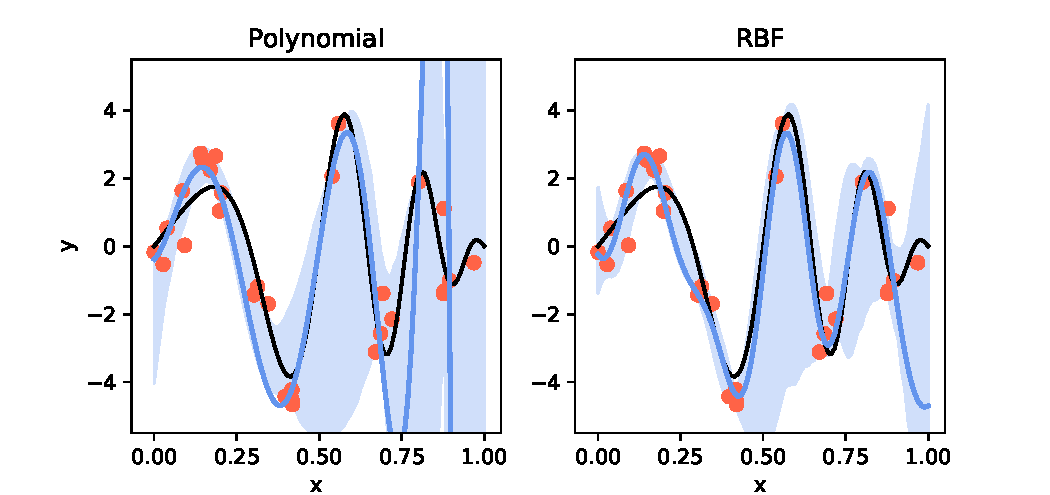
\includegraphics[width=0.7\textwidth]{code/A4b.pdf}

        \item Now for $n=300$ points, with 10-fold cross validation:
        \begin{itemize}
                \item Polynomial: $d = 23, ~ \lambda = 10^{-7}$ 
                \item RBF: $\gamma = 18.56, ~ \lambda = 10^{-5}$
        \end{itemize}
        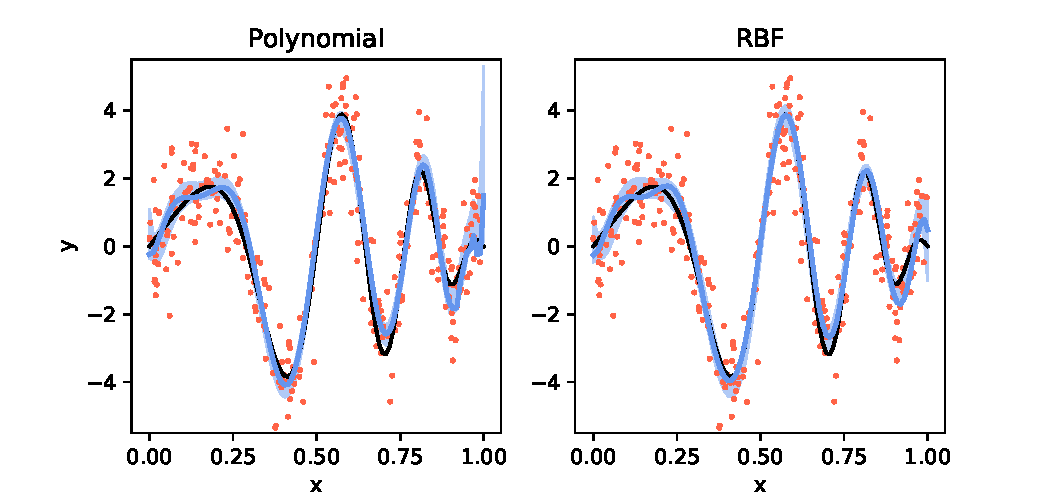
\includegraphics[width=0.7\textwidth]{code/A4d.pdf}

        \item The confidence interval is from 0.808-1160.627.
        Thus, there is high confidence that the polynomial kernel has a higher squared error than the RBF kernel.
        So there is statistically significant evidence to suggest that $\hat{f}_{rbf}$ is better than $\hat{f}_{poly}$.

\end{enumerate}

\begin{minted}{python}
import numpy as np
import matplotlib.pyplot as plt

# draw some x points
n = 30
np.random.seed(1)
x = np.random.uniform(size=n)
x.sort()

# simulate y data
f = lambda x: 4 * np.sin(np.pi*x) * np.cos(6*np.pi*x**2)
y = np.random.normal(f(x), 1)

class KernelRidgeRegressor():
    
    def __init__(self, kernel, param=1, lam=1):
        self.kernel = kernel
        self.param = param
        self.lam = lam
        
    def train(self, x, y, cv=10, param_range=None, lambdas=None, seed=1):
        
        # dictionary to save error as function of parameters
        errs = dict()
        
        # perform cross validation
        if cv:
            # how many points in each fold
            fold_len = len(x)//cv
            # randomly shuffle points
            idx = np.random.permutation(len(x))
            x_, y_ = x[idx], y[idx]
            
            # loop over the kernel parameter and lambda
            for param in param_range:
                for lam in lambdas:
                    se = 0 # variable to collect square error
                    # loop over the folds
                    for i in range(cv):
                        # draw training and test folds
                        xtrain, ytrain = x_[:-fold_len], y_[:-fold_len]
                        xtest, ytest = x_[-fold_len:], y_[-fold_len:]
                        # create the kernel matrix from the training data
                        K = self.kernel(*np.meshgrid(xtrain,xtrain), param)
                        # solve for alpha
                        alpha = np.linalg.solve((K + lam*np.identity(len(xtrain))), ytrain)
                        # use alpha and the kernel to calculate f_hat
                        fhat = np.vectorize(lambda z: alpha.dot(self.kernel(xtrain, z, param)))
                        # record sq error for the fold
                        se += np.mean((ytest - fhat(xtest))**2)
                        # roll points to prepare for the next fold
                        x_, y_ = np.roll(x_, fold_len), np.roll(y_, fold_len)
                    # save mean sq error for these parameter values
                    errs[(param,lam)] = se/len(x)
            # get the param and lambda corresponding to the lowest MSE
            self.param, self.lam = min(errs, key=errs.get)
        
        # set up the predict method using this data
        K = self.kernel(*np.meshgrid(x,x), self.param)
        alpha = np.linalg.solve((K + self.lam*np.identity(len(x))), y)
        self.predict = np.vectorize(lambda z: alpha.dot(self.kernel(x, z, self.param)))
        
    def plot_kernel(self, xmin=0, xmax=1, N=100):
        x = np.linspace(xmin, xmax, N)
        K = self.kernel(*np.meshgrid(x,x), self.param)
        plt.imshow(K)

# create a polynomial kernel ridge regressor
poly_kernel = KernelRidgeRegressor(lambda x, z, d: (1 + x*z)**d)
poly_kernel.train(x, y,
                  cv = len(x),
                  param_range = np.arange(1, 30, 1), 
                  lambdas = np.logspace(-6, 6, 13))
print(f'poly -- {poly_kernel.param:.2f}  {poly_kernel.lam}')

# create an RBF kernel ridge regressor
rbf_kernel = KernelRidgeRegressor(lambda x, z, gamma: np.exp(-gamma*(x-z)**2))
rbf_kernel.train(x, y,
                 cv = len(x),
                 param_range = np.linspace(1, 80, 100), 
                 lambdas = np.logspace(-6, 6, 13))
print(f'rbf  -- {rbf_kernel.param:.2f}  {rbf_kernel.lam}')


# Boot strapping
poly_bootstrap = []
rbf_bootstrap = []

grid = np.linspace(0, 1, 100)

B = 300
for i in range(B):
    
    idx = np.random.randint(len(x), size=len(x))
    x_, y_ = x[idx], y[idx]

    poly_kernel.train(x_, y_, cv=False)
    poly_bootstrap.append(poly_kernel.predict(grid))
    
    rbf_kernel.train(x_, y_, cv=False)
    rbf_bootstrap.append(rbf_kernel.predict(grid))

poly_5 = np.percentile(poly_bootstrap, 5, axis=0)
poly_95 = np.percentile(poly_bootstrap, 95, axis=0)

rbf_5 = np.percentile(rbf_bootstrap, 5, axis=0)
rbf_95 = np.percentile(rbf_bootstrap, 95, axis=0)


# Plotting
fig, (ax1, ax2) = plt.subplots(1, 2, figsize=(7, 3.3))

ax1.plot(grid, f(grid), c='k')
ax1.plot(grid, poly_kernel.predict(grid), c='cornflowerblue', lw=2)
ax1.fill_between(grid, poly_5, poly_95, color='cornflowerblue', alpha=0.3)
ax1.scatter(x, y, c='tomato')

ax2.plot(grid, f(grid), c='k')
ax2.plot(grid, rbf_kernel.predict(grid), c='cornflowerblue', lw=2)
ax2.fill_between(grid, rbf_5, rbf_95, color='cornflowerblue', alpha=0.3)
ax2.scatter(x, y, c='tomato')

ax1.set(ylim = (-5.5, 5.5),
        xlabel = 'x', 
        ylabel = 'y',
        title = 'Polynomial')
ax2.set(ylim = (-5.5, 5.5),
        xlabel = 'x',
        title = 'RBF')

# Finally, see if poly has statistically significant more err than rbf
n = 1300
np.random.seed(1)
x = np.random.uniform(size=n)
x.sort()
y = np.random.normal(f(x), 1)

vals = []

grid = np.linspace(0, 1, 100)

B = 300
for i in range(B):
    
    idx = np.random.randint(len(x), size=len(x))
    x_, y_ = x[idx], y[idx]

    poly_kernel.train(x_, y_, cv=False)
    poly_fhat = poly_kernel.predict(x_)
    
    rbf_kernel.train(x_, y_, cv=False)
    rbf_fhat = rbf_kernel.predict(x_)
    
    vals.append(np.mean((y_ - poly_fhat)**2 - (y_ - rbf_fhat)**2))
    
val_5 = np.percentile(vals, 5)
val_95 = np.percentile(vals, 95)
\end{minted}


\newpage
A.5

\begin{enumerate}
        \item We can minimize by setting the derivative equal to zero:
        \begin{align*}
                0 &= \frac{d}{dy} \sum_{i=1}^n (x_i-y)^T (x_i-y)
                = -2 \sum_{i=1}^n (x_i-y)
                = 2 \left( n \cdot y - \sum_{i=1}^n x_i \right)
                \quad \Longrightarrow \quad
                y = \frac{1}{n} \sum_{i=1}^n x_i
        \end{align*}

        \item Here is my k-means classifier that uses Lloyd's algorithm:
        \begin{minted}{python}
class KMeansClassifier():
    
    def __init__(self, k, centers=None):
        # number of clusters
        self.k = k
        # you can provide centers
        self.centers = centers
        # make sure correct number of centers provided
        if self.centers is not None:
            if len(centers) != k:
                raise ValueError('Centers must be array with len k')
                
    def predict(self, x):
        return ((x[:,None,:] - self.centers)**2).sum(axis=-1).argmin(axis=1)
    
    def score(self, x):
        return ((x[:,None,:] - self.centers)**2).sum(axis=-1).min(axis=1).mean()
    
    def train(self, x, return_scores=False):
        
        # start with random centers
        self.centers = np.random.permutation(x)[:self.k]
        
        # initial labels
        labels = -np.ones(len(x))
        labels_new = self.predict(x)
        
        # list of scores
        scores = [self.score(x)]
        
        # loop training until labels don't change
        while np.any(labels != labels_new):
            
            # use new labels
            labels = labels_new
            # calculate new centers
            self.centers = np.array([data[labels == k].mean(axis=0) for k in range(self.k)])
            # generate new labels
            labels_new = self.predict(x)
            
            # save score
            scores.append(self.score(x))
            
        if return_scores:
            return scores
        \end{minted}
        Here is some data and a plot to demonstrate it works:
        \begin{minted}{python}
np.random.seed(10)
data = np.vstack((np.random.normal(0,size=(300,2)),
                  np.random.normal(1,size=(300,2)),
                  np.random.normal(-1.5,size=(300,2)),
                  np.random.normal([-1,1],size=(300,2))))
        \end{minted}
        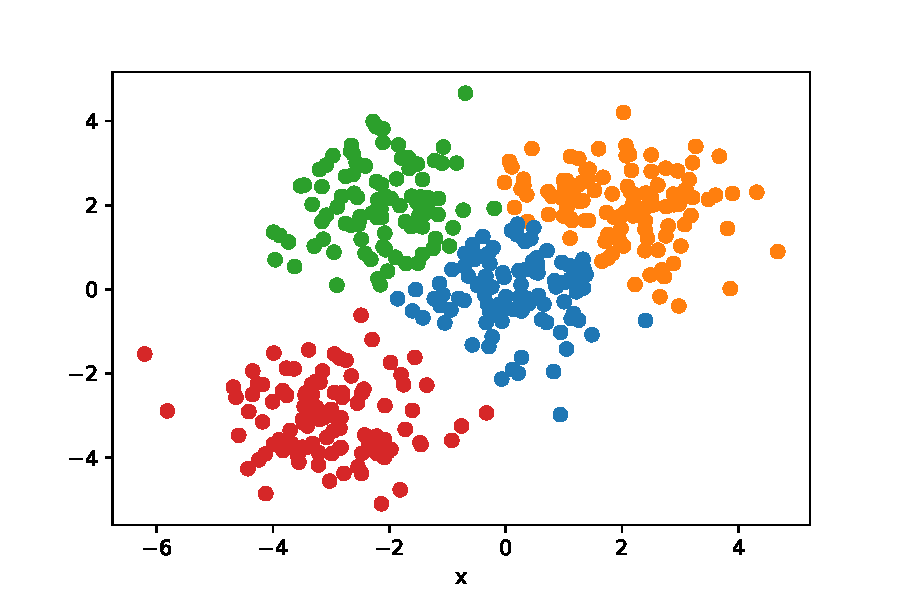
\includegraphics[width=0.5\textwidth]{code/kmeans_ex.pdf}

        \item Here I apply the clustering algorithm to MNIST data with $k=10$.
        First the objective: \\
        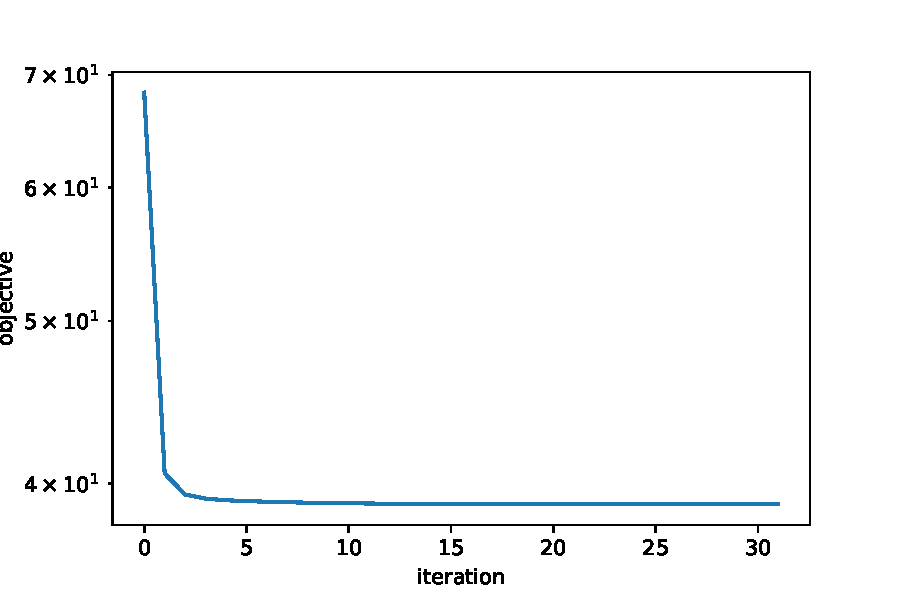
\includegraphics[width=0.6\textwidth]{code/A5c_objective.pdf} \\
        Now the centers: \\
        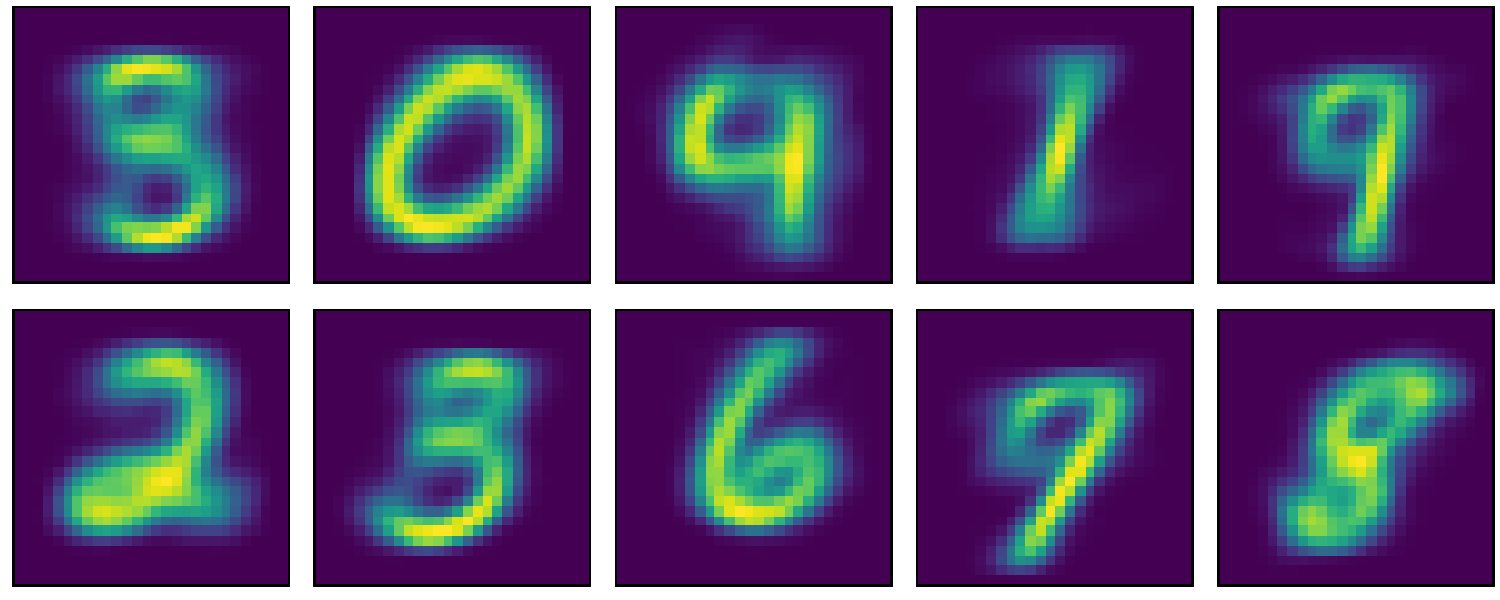
\includegraphics[width=\textwidth]{code/A5c_centers.pdf} \\
        \begin{minted}{python}
from mnist import MNIST

def load_dataset():
    mndata = MNIST('../../../python-mnist/data/')
    X_train, labels_train = map(np.array, mndata.load_training())
    X_test, labels_test = map(np.array, mndata.load_testing())
    X_train = X_train/255.0
    X_test = X_test/255.0
    
    return X_train, labels_train, X_test, labels_test

X_train, Y_train, X_test, Y_test = load_dataset()

kmeans = KMeansClassifier(10)
scores = kmeans.train(X_train, return_scores=True)
        \end{minted}

        \item Below are the training and test errors as a function of $k$.
        It looks like increasing $k$ continues to decrease the training error.
        The test error is decreasing as well, but looks like it is approaching a lower bound. \\
        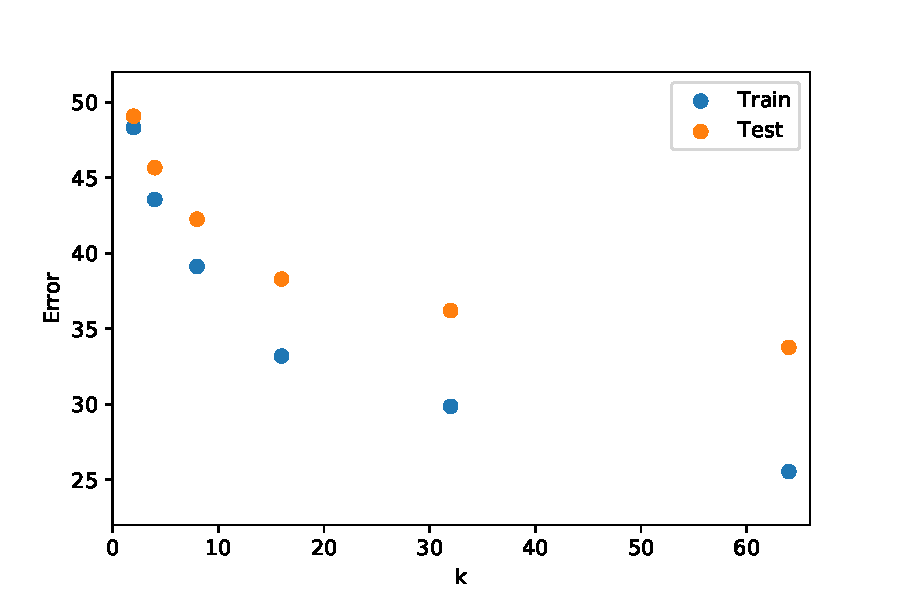
\includegraphics[width=0.5\textwidth]{code/A5d.pdf}
        \begin{minted}{python}
train_err = dict()
test_err = dict()
for k in [2,4,8,16,32,64]:
    kmeans = KMeansClassifier(k)
    kmeans.train(X_train[:1000])
    train_err[k] = kmeans.score(X_train[:1000])
    test_err[k] = kmeans.score(X_test[:1000])
        \end{minted}
\end{enumerate}


\newpage
\section*{Intro to sample complexity}

B1

\begin{enumerate}
        \item Since the only two outcomes are 0 or 1, the expectation value $R$ is the probability of getting a 1.
        Thus, if $R > \epsilon$, then $P(0) = 1 - P(1) \leq 1 - \epsilon$.
        Now, if we draw $n$ times, we get $P(0, n~\mathrm{times}) \leq (1- \epsilon)^n$.
        Applying the given inequality, we have $P(\hat{R}_n(f)=0) \leq e^{-n\epsilon}$.

        \item Let $A_i$ denote the case that $f_i$ meets the conditions.
        Then from the result of a, $P(A_i) \leq e^{-n\epsilon}$.
        Then using the union bound:
        \begin{align*}
                P(\cup_i A_i) \leq \sum_i P(A_i) \leq \sum_i e^{-n\epsilon} = |\mathcal{F}| e^{-\epsilon n}
        \end{align*}

        \item Using simple algebraic manipulations,
        \begin{align*}
                |\mathcal{F}| e^{-\epsilon n} &\leq \delta \\
                e^{-\epsilon n} &\leq \frac{\delta}{|\mathcal{F}|} \\
                -\epsilon n &\leq \log \frac{\delta}{|\mathcal{F}|} \\
                \epsilon &\geq \frac{1}{n} \log \frac{|\mathcal{F}|}{\delta}
        \end{align*}
        Thus the minimum value for $\epsilon$ is $\epsilon = \frac{1}{n} \log \frac{|\mathcal{F}|}{\delta}$.

        \item Assume $\hat{R}_n(\hat{f}) = 0$, then $P \leq |\mathcal{F}| e^{-\epsilon n} = \delta$ that $R(\hat{f}) - R(f^*) \geq \epsilon$, if we choose $\epsilon = \frac{1}{n} \log \frac{|\mathcal{F}|}{\delta}$ as in c.
        We can then reverse the inequality by taking the complement.
        I.e. there is probability $1 - \delta$ that $R(\hat{f}) - R(f*) \leq \frac{1}{n} \log \frac{|\mathcal{F}|}{\delta}$.
        
        
\end{enumerate}

\newpage
\section*{Perceptron}

B2

\begin{enumerate}
        \item Referring to the answer of A2.b.b, we can use the derivatives of the maximum for each point.
        When this is zero, the gradient is zero, so we only need to care about the points that are misclassified.
        The gradient of $\ell$ is
        \begin{align*}
                \frac{\partial \ell}{\partial w} = 
                \frac{1}{n} \sum_{i=1}^n -y_i x_i \, \mathbf{1}\{y_i(w \cdot x_i) < 0\},
        \end{align*}
        and we update like $\tilde{w} \leftarrow \tilde{w} - \eta \frac{\partial \ell}{\partial w}$.

        \item Let's do SGD with a batch size of 1.
        Then
        \begin{align*}
                \frac{\partial \ell}{\partial w} = 
                -y_i x_i \, \mathbf{1}\{y_i(w \cdot x_i) < 0\}.
        \end{align*}
        Thus, when we make a mistake, we update $w$ like
        \begin{align*}
                w_{t+1} = w_t + \eta y_i x_i.
        \end{align*}
        If we set $\eta = 1$, then we have
        \begin{align*}
                w_{t+1} = w_t + y_i \, x_i.
        \end{align*}
        As $y_i = \pm 1$, this is exactly the perceptron algorithm.

        \item This loss doesn't have a margin, so it treats any plane that separates the data as equally good.
        However, we typically want a plane that has a maximum distance from both data classes, as this will generalize better.
        Otherwise, we may select a plane that \textit{barely} separates the classes, and future points may fall on either side.
\end{enumerate}

\newpage
\section*{Neural Network for MNIST}

A6

\begin{enumerate}
        \item I trained the shallow network for 1200 epochs: \\
        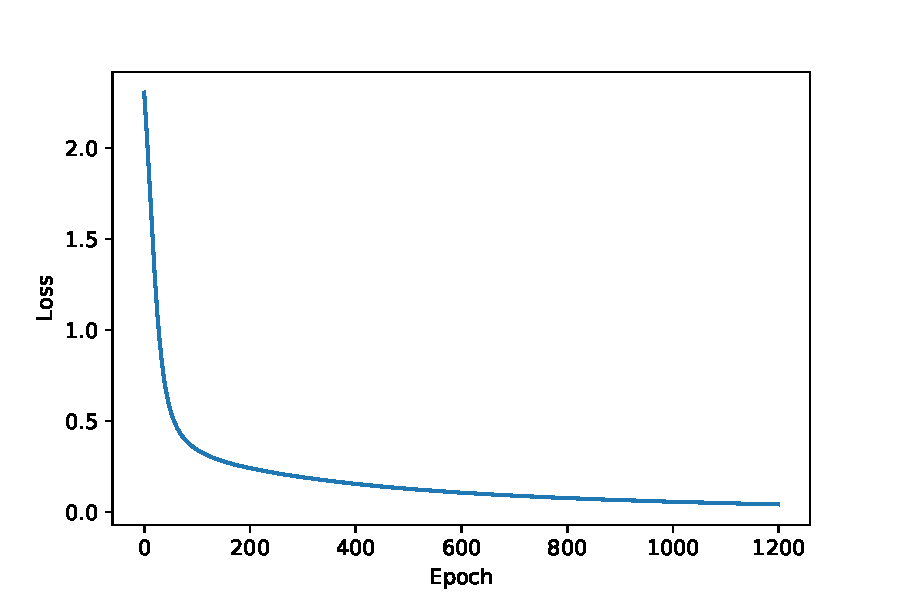
\includegraphics[width=0.5\textwidth]{code/A6a.pdf} \\
        The final test loss is 0.106 and the test accuracy is 0.969.
        Here is the code for the shallow network:
        \begin{minted}{python}
import torch
from torch.nn.functional import relu, cross_entropy
from torch.optim import Adam

from mnist import MNIST

def load_dataset():
    mndata = MNIST('../../../python-mnist/data/')
    X_train, labels_train = map(np.array, mndata.load_training())
    X_test, labels_test = map(np.array, mndata.load_testing())
    X_train = X_train/255.0
    X_test = X_test/255.0
    
    return X_train, labels_train, X_test, labels_test

X_train, Y_train, X_test, Y_test = load_dataset()

X_train = torch.from_numpy(X_train).float()
Y_train = torch.from_numpy(Y_train).long()
X_test = torch.from_numpy(X_test).float()
Y_test = torch.from_numpy(Y_test).long()

def weights(n, m):
    return (2/np.sqrt(m)*torch.rand(size=(n,m)) - 1/np.sqrt(m)).requires_grad_()
def bias(n, m):
    return (2/np.sqrt(m)*torch.rand(size=(n,1)) - 1/np.sqrt(m)).requires_grad_()

    k = 10
d = 784
h = 64

# initialize parameters
W0 = weights(h, d)
b0 = bias(h, d)
W1 = weights(k, h)
b1 = bias(k, h)

# definte the neural network
def F1(x):
    y_hat = torch.matmul(W0, x.T) + b0
    y_hat = relu(y_hat)
    y_hat = torch.matmul(W1, y_hat) + b1
    return y_hat.T

# function to calculate accuracy
def accuracy(y_hat, y):
    return len(y[y_hat.argmax(axis=1) == y]) / len(y)

# make initial predictions
y_hat = F1(X_train)

# initialize Adam optimizer
optim = Adam((W0, b0, W1, b1))

# train until accuracy > 0.99
losses = []
for i in range(1200):

    # predict
    y_hat = F1(X_train)
    # calculate loss
    loss = cross_entropy(y_hat, Y_train)
    losses.append(loss.data.numpy())
    # zero out gradients
    optim.zero_grad()
    # calculate new gradients
    loss.backward()
    # step optimizer forward 
    optim.step()

print(len(losses),'epochs')
    
y_hat_test = F1(X_test)
print('test loss ', cross_entropy(y_hat_test, Y_test).data.numpy())
print('test accuracy', accuracy(y_hat_test, Y_test))

# calculate the number of parameters
print('nparams', torch.numel(W0) + torch.numel(b0) + torch.numel(W1) + torch.numel(b1))
        \end{minted}

        \newpage
        \item I trained the deep network trained for 1200 epochs: \\
        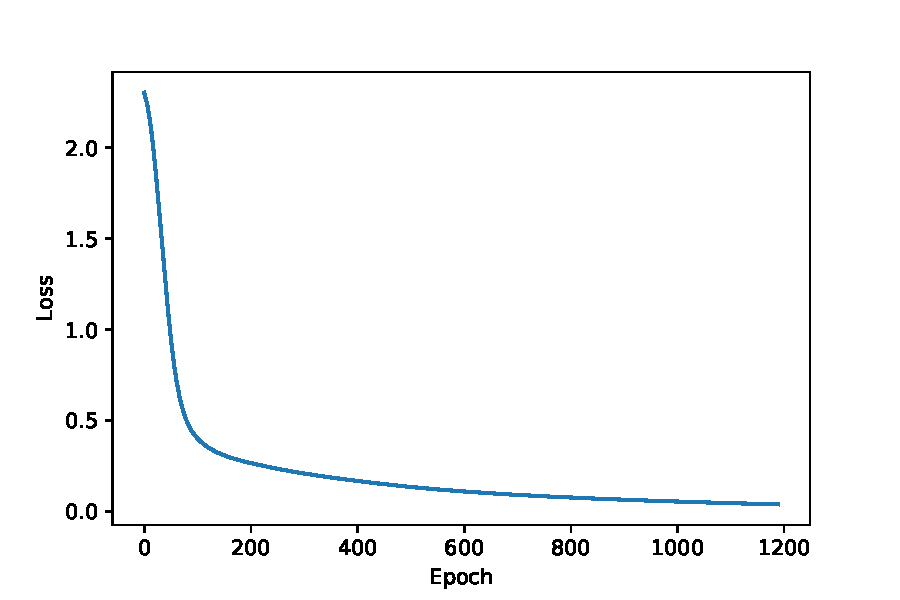
\includegraphics[width=0.5\textwidth]{code/A6b.pdf} \\
        The test loss is 0.135 and the accuracy is 0.964, both of which are a little worse than the shallow network.
        Here is the code for the deep network:
        \begin{minted}{python}
import torch
from torch.nn.functional import relu, cross_entropy
from torch.optim import Adam

from mnist import MNIST

def load_dataset():
    mndata = MNIST('../../../python-mnist/data/')
    X_train, labels_train = map(np.array, mndata.load_training())
    X_test, labels_test = map(np.array, mndata.load_testing())
    X_train = X_train/255.0
    X_test = X_test/255.0
    
    return X_train, labels_train, X_test, labels_test

X_train, Y_train, X_test, Y_test = load_dataset()

X_train = torch.from_numpy(X_train).float()
Y_train = torch.from_numpy(Y_train).long()
X_test = torch.from_numpy(X_test).float()
Y_test = torch.from_numpy(Y_test).long()

def weights(n, m):
    return (2/np.sqrt(m)*torch.rand(size=(n,m)) - 1/np.sqrt(m)).requires_grad_()
def bias(n, m):
    return (2/np.sqrt(m)*torch.rand(size=(n,1)) - 1/np.sqrt(m)).requires_grad_()

    k = 10
d = 784
h0 = 32
h1 = 32

# initialize parameters
W0 = weights(h0, d)
b0 = bias(h0, d)
W1 = weights(h1, h0)
b1 = bias(h1, h0)
W2 = weights(k, h1)
b2 = bias(k, h1)

# definte the neural network
def F2(x):
    y_hat = torch.matmul(W0, x.T) + b0
    y_hat = relu(y_hat)
    y_hat = torch.matmul(W1, y_hat) + b1
    y_hat = relu(y_hat)
    y_hat = torch.matmul(W2, y_hat) + b2
    return y_hat.T

# function to calculate accuracy
def accuracy(y_hat, y):
    return len(y[y_hat.argmax(axis=1) == y]) / len(y)

# make initial predictions
y_hat = F2(X_train)

# initialize Adam optimizer
optim = Adam((W0, b0, W1, b1, W2, b2))

# train until accuracy > 0.99
losses = []
#while accuracy(y_hat, Y_train) < 0.99:
for i in range(1200):

    # predict
    y_hat = F2(X_train)
    # calculate loss
    loss = cross_entropy(y_hat, Y_train)
    losses.append(loss.data.numpy())
    # zero out gradients
    optim.zero_grad()
    # calculate new gradients
    loss.backward()
    # step optimizer forward 
    optim.step()
    
print(len(losses),'epochs')
    
y_hat_test = F2(X_test)
print('test loss ', cross_entropy(y_hat_test, Y_test).data.numpy())
print('test accuracy', accuracy(y_hat_test, Y_test))

# calculate the number of parameters
print('nparams', torch.numel(W0) + torch.numel(b0) 
                    + torch.numel(W1) + torch.numel(b1) 
                    + torch.numel(W2) + torch.numel(b2))
        \end{minted}

        \item 
        Shallow: parameters - 50890 \quad accuracy - 0.969 \\
        Deep: ~~ parameters - 26506 \quad accuracy - 0.964 \\
        The deep network has more parameters but is slightly less accurate.
        The shallow network, which has almost twice the number of parameters, is able to learn the structure of the data better and generalize better.
\end{enumerate}

\newpage

\section*{PCA}
A.7

\begin{enumerate}
        \item 
        $\lambda_1 = 5.148 \\
        \lambda_2 = 3.730 \\
        \lambda_{10} = 1.250 \\
        \lambda_{30} = 0.365 \\
        \lambda_{50} = 0.170 \\
        \sum_i \lambda_i = 52.834$ \\ \, \\
        The code follows:
        \begin{minted}{python}
from mnist import MNIST

def load_dataset():
    mndata = MNIST('../../../python-mnist/data/')
    X_train, labels_train = map(np.array, mndata.load_training())
    X_test, labels_test = map(np.array, mndata.load_testing())
    X_train = X_train/255.0
    X_test = X_test/255.0
    
    return X_train, labels_train, X_test, labels_test

X_train, Y_train, X_test, Y_test = load_dataset()

ndata = 50000
X_train = X_train[:ndata]
Y_train = Y_train[:ndata]
X_test = X_test[:ndata]
Y_test = Y_test[:ndata]

Sigma_train = 1/ndata * (X_train - X_train.mean(axis=0)).T @ (X_train - X_train.mean(axis=0))

evals = np.linalg.eigvalsh(Sigma_train)[::-1]
print(evals[[0,1,9,29,49]])
print(evals.sum())
        \end{minted}

        \item Let the eigenvector of $\Sigma$ corresponding to the eigenvalue $\lambda_i$ be denoted $u_i$.
        Then we can approximate $x$ via the projection onto the first $k$ eigenvectors: $ x = \mu + \sum_{i=1}^k u_i u_i^T (x - \mu) $.

        \newpage
        \item Here is the reconstruction error: \\
        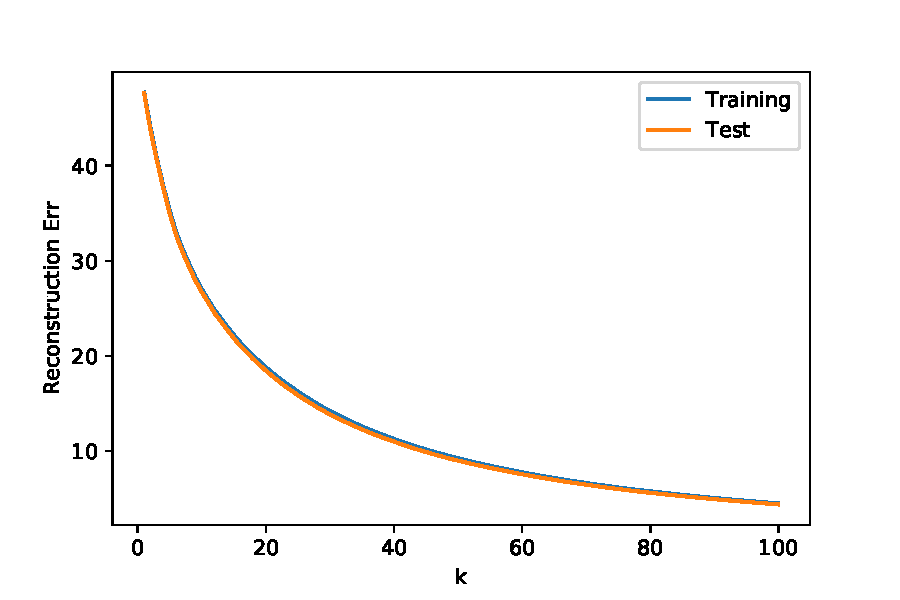
\includegraphics[width=0.6\textwidth]{code/A7c_err.pdf} \\
        and here is the second plot \\
        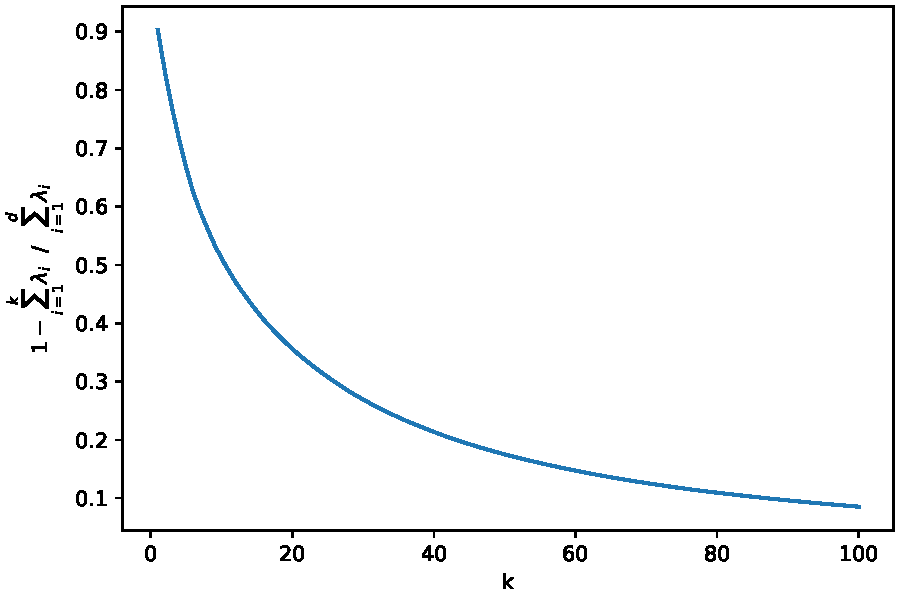
\includegraphics[width=0.6\textwidth]{code/A7c_evals.pdf} \\
        Here is the code to produce these plots:
        \begin{minted}{python}
evals, evecs = np.linalg.eigh(Sigma_train)
evals, evecs = evals[::-1], evecs[:,::-1]

eigproj = lambda X, k: mu + (evecs[:,:k] @ (evecs[:,:k].T @ (X - mu).T)).T
recon_err = lambda X, k: ((X - eigproj(X, k))**2).sum(axis=1).mean()
k = np.arange(1,101)
train_errs = [recon_err(X_train, ki) for ki in k]
test_errs = [recon_err(X_test, ki) for ki in k]

plt.plot(k, train_errs, label='Training')
plt.plot(k, test_errs, label='Test')
plt.legend()
plt.xlabel('k')
plt.ylabel('Reconstruction Err')

fig,ax = plt.subplots(constrained_layout=True)
ax.plot(k, [1 - evals[:ki].sum()/evals.sum() for ki in k])
ax.set_xlabel('k')
ax.set_ylabel('$1 - \sum_{i=1}^k \lambda_i ~~ / ~~ \sum_{i=1}^d \lambda_i$')
        \end{minted}

        \newpage
        \item Here are the top 10 eigenvectors: \\
        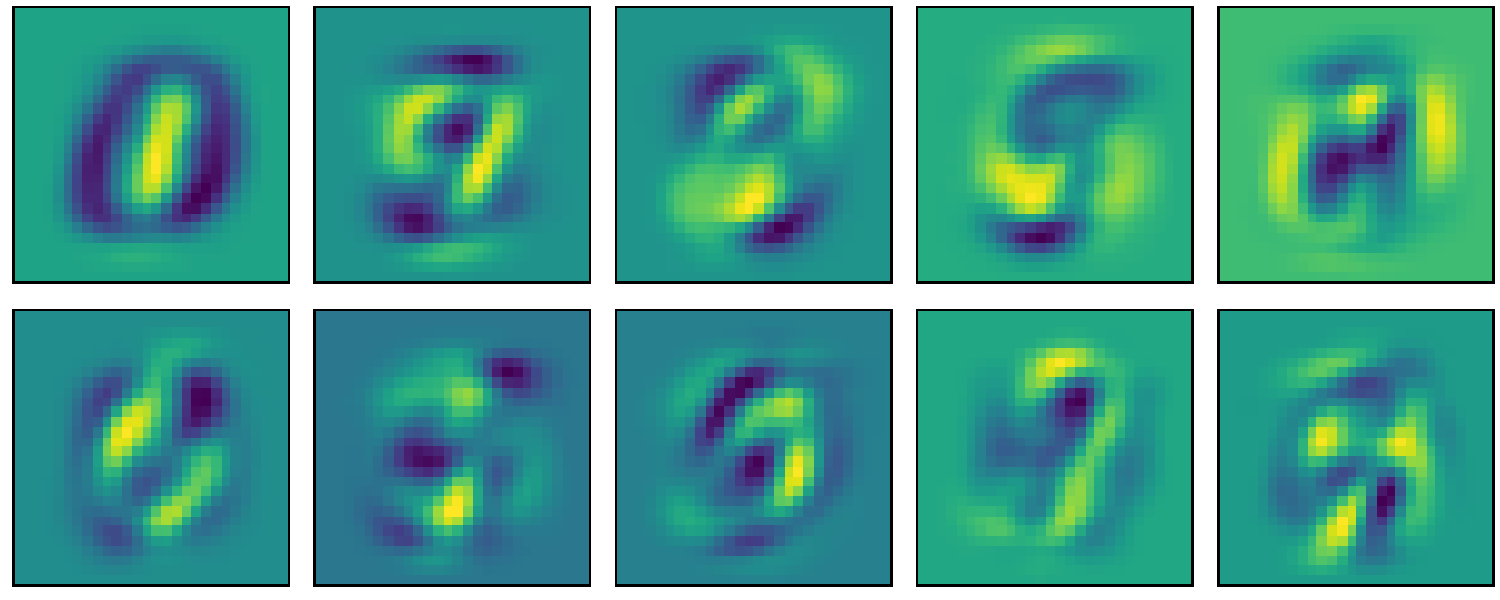
\includegraphics[width=\textwidth]{code/A7d.pdf} \\
        A few of these directly resemble the digits 0, 1, 9, and 6.
        All of them capture different edges and curves that can be used to build the various digits 0 -- 9. \\
        Here is the code:
        \begin{minted}{python}
fig, axes = plt.subplots(2, 5, figsize=(10,4), constrained_layout=True)

axes = axes.flatten()

for i,ax in enumerate(axes):
    ax.imshow(evecs[:,i].reshape(28,28))
    ax.set(xticks=[],yticks=[])
        \end{minted}

        \item \, \\
        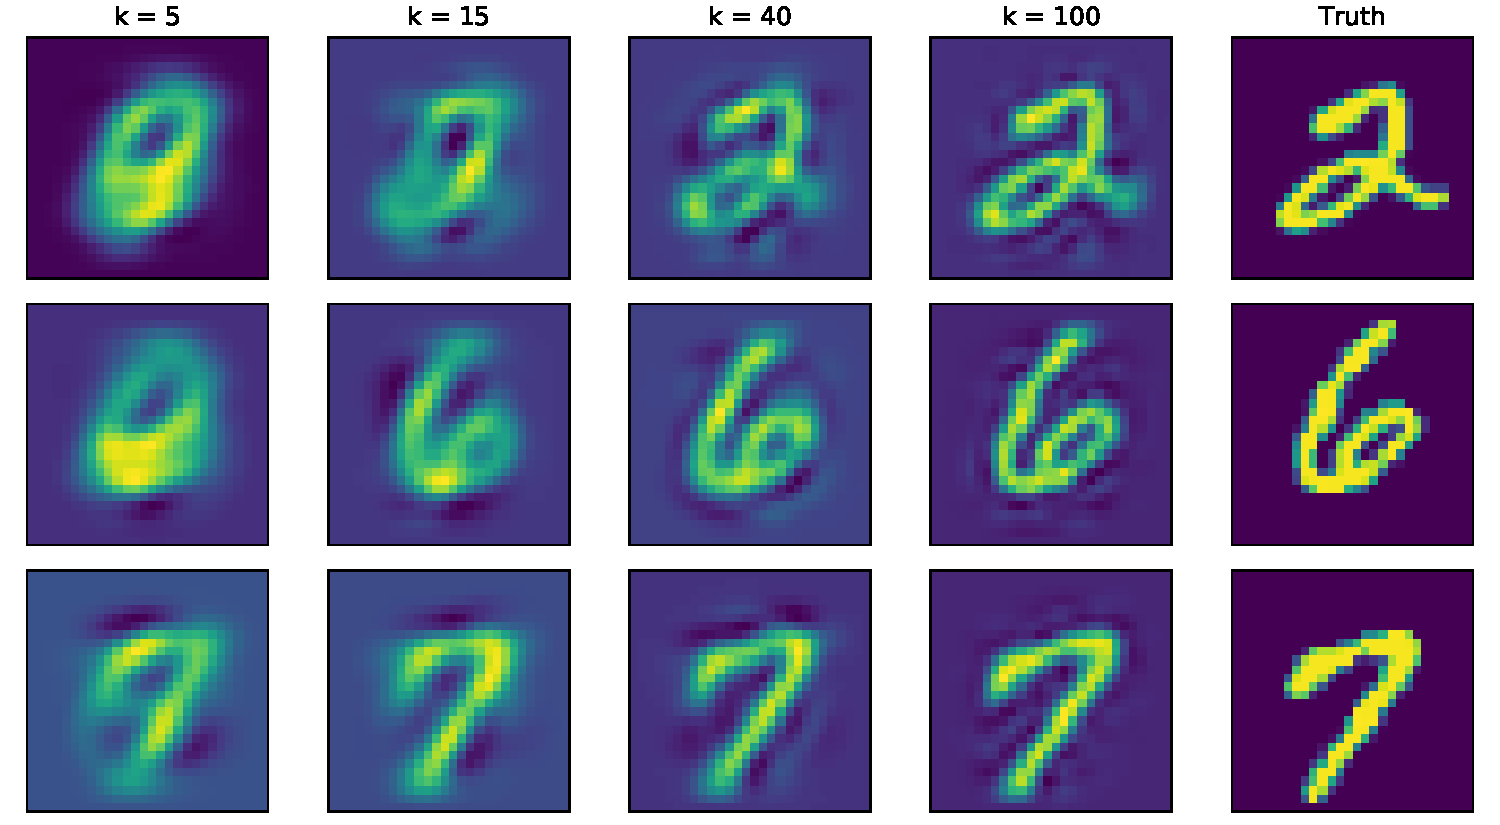
\includegraphics[width=\textwidth]{code/A7e.pdf} \\
        Interestingly, the 2 and 6 digits look almost identical when $k=5$, but the $7$ is clearly differentiated.
        It takes 15 components to clearly differentiate the digits.
        By 40 components, each digit is fully and clearly formed, and adding additional components just sharpens the images.
        \begin{minted}{python}
fig, axes = plt.subplots(3, 5, figsize=(10,5.5), constrained_layout=True)

yidx = [5,13,15]
k = [5,15,40,100]

for i,yi in enumerate(yidx):
    for j,ax in enumerate(axes[i,:-1]):
        xproj = eigproj(X_train[yi], k[j])
        ax.imshow(xproj.reshape(28,28))
        if i == 0:
            ax.set_title(f'k = {k[j]}')
    axes[i,-1].imshow(X_train[yi].reshape(28,28))
    
axes[0,-1].set_title('Truth')

for i,ax in enumerate(axes.flatten()):
    ax.set(xticks=[],yticks=[])
        \end{minted}
\end{enumerate}




\end{document}
